% \documentclass[11pt]{article}
\documentclass[12pt,a4paper,oneside,draft]{article}
\usepackage[margin=1in]{geometry}
\usepackage{amsmath}
\usepackage{amsthm}
\usepackage{amssymb}
\usepackage{graphicx}
\usepackage{hyperref}
\usepackage[latin1]{inputenc}
\usepackage{mathtools}
\usepackage{tikz}
\usetikzlibrary{trees}
\DeclarePairedDelimiter{\ceil}{\lceil}{\rceil}
\DeclarePairedDelimiter{\floor}{\lfloor}{\rfloor}

\title{MTH 361, Homework Assignment 2} 
\author{Nurseiit Abdimomyn -- 20172001}
\date{21/04/2020}

\begin{document}
\maketitle

\begin{enumerate}
  \item
    \begin{itemize}
      \item
        Find the adjacent matrix of network (a).
        \newline
        \newline
        $A = \begin{pmatrix}
              0&1&0&0&1\\
              0&0&1&0&0\\
              1&0&0&0&1\\
              0&1&1&0&0\\
              0&0&0&0&0\\
            \end{pmatrix}$
        \newline
      \item
        Find the incident matrix of network (b).
        \newline
        \newline
        $B = \begin{pmatrix}
              1&0&1&0&0\\
              0&1&1&0&0\\
              0&0&0&1&0\\
              0&1&1&1&1\\
            \end{pmatrix}$
        \newline
      \item
        Find the adjacent matrix for the network generated when we project
        the network (b) into its black vertices.
        \newline
        \newline
        $A' = \begin{pmatrix}
              0&0&1&0&0\\
              0&0&1&1&1\\
              1&1&0&1&1\\
              0&1&1&0&1\\
              0&1&1&1&0\\
            \end{pmatrix}$
        \newline
    \end{itemize}
  \item
    \begin{itemize}
      \item
        A 3-regular graph must have an even number of nodes.
        \begin{proof}
          By Handshaking lemma we have sum of all degrees: $$\sum_{v \in V} deg(v) = 2 * |E|$$
          and by the defition of regular graphs, 3-regular graph has sum of all degrees
          $$\sum_{v \in V} deg(v) = 3 * |V|.$$
          Thus, we have $$3 * |V| = 2 * |E|$$ which implies that $|V| = 2 * k$ for some $k$.
        \end{proof}
      \item
        The average degree of a tree is strictly less than 2.
        \begin{proof}
          Via Handshaking lemma, the average degree of a graph is as follows:
            $$c = \frac{1}{|V|} * \sum_{v \in V} deg(v) = \frac{2 * |E|}{|V|}.$$
          By definition, the following holds true for all trees: $$|E| = |V| - 1.$$
          Thus, by substituting $|V|$:
            $$c = \frac{2 * (|V| - 1)}{|V|} = 2 - \frac{1}{|V|} < 2$$
        \end{proof}
    \end{itemize}
  \item
    Consider a network which is simple (it contains no multiedges or self-edges)
    and consists of $n$ nodes in a single component.
    \newline
    (i) What is the maximum possible number of edges it could have?
    \newline
    (ii) What is the minimum possible edges if could have?
    \newline
    Explain how you give the answer by providing the corresponding figures of networks.
    \begin{itemize}
      \item [(i) ]
        One could draw an edge between every of the $n$ nodes of the graph to
        form a \textit{complete graph} with $|E| = \frac{n * (n - 1)}{2}$.
        \newline
        \begin{center}
          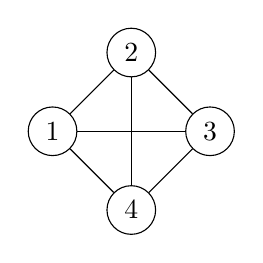
\begin{tikzpicture}
            [scale=.5,auto=left,every node/.style={circle,draw=black}]

            \node (n4) at (10, 6) {1};
            \node (n5) at (12, 8) {2};
            \node (n6) at (14, 6) {3};
            \node (n7) at (12, 4) {4};

            \foreach \from/\to in {n4/n5,n4/n6,n4/n7,n5/n6,n5/n7,n6/n7}
              \draw (\from) -- (\to);

          \end{tikzpicture}
          $$|E| = \frac{4 * (4 - 1)}{2} = 6.$$
        \end{center}
      \item [(ii) ]
        One could form a \textit{tree graph} with $n$ nodes to get $|E| = n - 1$.
        \newline
        \begin{center}
          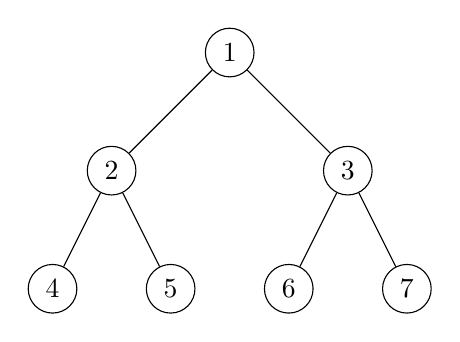
\begin{tikzpicture}[level distance=1.5cm,
            level 1/.style={sibling distance=3cm},
            level 2/.style={sibling distance=1.5cm}, every node/.style={circle,draw=black}]
            \node {1}
              child {node {2}
                child {node {4}}
                child {node {5}}
              }
              child {node {3}
              child {node {6}}
                child {node {7}}
              };
          \end{tikzpicture}
          $$|E| = 7 - 1 = 6.$$
        \end{center}
    \end{itemize}
  \item
    \begin{itemize}
      \item [(i) ] How do $n$, $m$, and $f$ change when we add a single vertex to such a network 
      along with a single edge attaching it to an existing vertex?
      \newline
        $$n \implies n + 1; m \implies m + 1; f \implies f;$$
      One can't form any "face" with $1$ new edge and $1$ new node only.
      \newline
      \newline
      \item [(ii) ] How do $n$, $m$, and $f$ change when we add a single edge between two existing vertices
      (or a self-edge attached to just one vertex), in such a way as to maintain planarity of the network?
      \newline
        $$n \implies n; m \implies m + 1; f \implies f + 1;$$
      By adding an edge while maintaining planarity of the graph we will bound a new area and form a new "face".
      \newline
      \newline
      \item [(iii) ] What are the values of $n$, $m$, and $f$ for a network with a single vertex and no edges?
        $$n \implies 1; m \implies 0; f \implies 1;$$
      With no "faces" except the outer one.
      \newline
      \newline
      \item [(iv) ] Hence by induction prove a general relation between n, m, and f for all
      connected planar networks.
      \newline
      \newline
      Let's prove Euler's identity for planar graphs as $n - m + f = 2$, where
      $n = |V|, m = |E|, f = |\textit{faces}|$.
      \newline
      (1.) Basic step of induction is given in (iii):
        $$n \implies 1; m \implies 0; f \implies 1;$$
        $$\text{so, } n - m + f = 1 - 0 + 1 = 2; \square$$
      \newline
      (2.) Induction step is given in (i) and (ii) by assuming $n - m + f = 2$ is \textit{true}:
        $$\text{(i): } n \implies n + 1; m \implies m + 1; f \implies f;$$
        $$\text{so, } (n + 1) - (m + 1) + f = n - m + f = 2;$$
        $$\text{(ii): } n \implies n; m \implies m + 1; f \implies f + 1;$$
        $$\text{so, } n - (m + 1) + (f + 1) = n - m + f = 2; \square$$
      \newline
      \item [(v) ] Now suppose that our network is simple. Show that the mean degree $c$ of a simple,
      connected, planar network is strictly less than \textit{six}.
      \newline
      \begin{proof}
        By Handshaking lemma, we know that mean degree is
          $$c = \frac{1}{|V|} * \sum_{v \in V} deg(v) = \frac{2 * |E|}{|V|} = \frac{2 * m}{n},$$
        and we proved $n - m + f = 2$ in (iv).
        \newline
        Similar to Handshaking lemma, we know for sum of degress of all faces:
          $$\sum_{i} deg(f_i) = 2 * |E| = 2 * m.$$
        From there, because our graphs are all simple, the smallest possible degree of a face
        would be $3$, so:
          $$\sum_{i} 3 \leq \sum_{i} deg(f_i) \implies 3 * f \leq 2 * m.$$
        Thus, by solving for $f$ in $n - m + f = 2 \implies f = 2 + m - n$ we get:
          $$3 * f \leq 2 * m \implies 3 * (2 + m - n) \leq 2 * m \implies m \leq 3*n - 6.$$
        Further, by substituting the above to the equation for mean degree $c$:
          $$c = \frac{2 * m}{n} \leq \frac{2*(3*n - 6)}{n} \implies c \leq 6 - \frac{12}{n}.$$
        Which for all $n \neq 0$ it's true that $c < 6.$
      \end{proof}
    \end{itemize}
    \item
      What is the difference between a 2-component and a 2-core?
      Draw a small network that has one 2-core but two 2-components.
      \newline
      \newline
      2-component is a maximal subset of vertices s.t. each one's reachable from each others
      by at least $2$ \textit{vertex-independent} paths.
      \newline
      While 2-core is a maximal subset of vertices s.t. each one's connected to at least
      $2$ others in the subset.
      \newline
      \begin{center}
        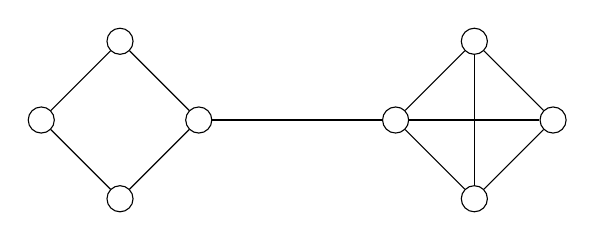
\begin{tikzpicture}
          [scale=.5,every node/.style={circle,draw=black}]
          \node (n1) at (1,6) {};
          \node (n2) at (3,8) {};
          \node (n3) at (5,6) {};
          \node (n8) at (3,4) {};

          \node (n4) at (10, 6) {};
          \node (n5) at (12, 8) {};
          \node (n6) at (14, 6) {};
          \node (n7) at (12, 4) {};

          \foreach \from/\to in {n1/n2,n1/n8,n8/n3,n2/n3,n3/n4,n4/n5,n4/n6,n4/n7,n5/n6,n5/n7,n6/n7}
            \draw (\from) -- (\to);

        \end{tikzpicture}
        \newline
        One 2-core, 2-component (left) and one 3-core, 2-component (right).
      \end{center}
    \item
      Show that the edge connectivity of nodes A and B in the network is 2.
      \begin{proof}
        First, we can see that there are not any \textit{edge cut size} less than $2$ in a given graph.
        Thus, there must be \textit{at least} $2$ edge-independent paths between two vertices $A$ and $B$.
        So, $2 \leq \text{edge connectivity}$.
        \newline
        Let's assume there to be exactly $2$ edge-independent paths from $A$ to $B$. Which'd simply mean
        that \textit{at least} we'd have to remove \textit{one} edge from each of the paths for $A$ and $B$
        to disconnect. This implies that edge cut size of the graph is \textit{at least} $2$.
        So, $2 \geq \text{edge connectivity}$.
          $$2 \leq \text{edge connectivity} \leq 2 \implies \text{edge connectivity} = 2.$$
      \end{proof}
\end{enumerate}

\end{document}
